\documentclass[a4paper,12pt]{article}
\usepackage[a4paper,top=1.3cm,bottom=2cm,left=1.5cm,right=1.5cm,marginparwidth=0.75cm]{geometry}
%%% Работа с русским языком
\usepackage{cmap}					% поиск в PDF
\usepackage{mathtext} 				% русские буквы в фомулах
\usepackage[T2A]{fontenc}			% кодировка
\usepackage[utf8]{inputenc}			% кодировка исходного текста
\usepackage[english,russian]{babel}	% локализация и переносы

\usepackage{graphicx}
\usepackage{mathtools}
\usepackage{wrapfig}
\usepackage{tabularx}
\usepackage{amssymb}
\usepackage{hyperref}
\usepackage[rgb]{xcolor}
\hypersetup{colorlinks=true,urlcolor=blue}
\setcounter{secnumdepth}{0}
%% Шрифты
\usepackage{euscript}	 % Шрифт Евклид
\usepackage{amsmath}
\usepackage{mathtools}
%%% Заголовок
\author{Tsvetkova Amelia}
\title{Лабораторная работа по общей физике}

\date{\today}
\begin{document}
\begin{titlepage}
    \newpage
    \begin{center}
    {\large МОСКОВСКИЙ ФИЗИКО-ТЕХНИЧЕСКИЙ ИНСТИТУТ (НАЦИОНАЛЬНЫЙ ИССЛЕДОВАТЕЛЬСКИЙ УНИВЕРСИТЕТ)}
    \vspace{1cm}

    {\largeФизтех-школа аэрокосмических технологий}
    \vspace{6em}
    \end{center}
    
    \vspace{1.2em}

    \begin{center}
    \Large Лабораторные работы №5.2.2 и №5.2.3 \\
    Изучение спектров атомов водорода и дейтерия
    Изучение молекулярного спектра йода
    \linebreak
    \end{center}
    
    \vspace{11em}
    
    \begin{flushright}
                       {\large Работу выполнила\\
                       Цветкова Амелия Антоновна\\
                       Б03-305 }
    \end{flushright}

    \vspace{\fill}

    \begin{center}
    Долгопрудный, 2025
    \end{center}

    \end{titlepage}

\section{Цели работы}
\begin{enumerate}
    \item Исследовать спектральные закономерности в оптических спектрах водорода;
    \item По результатам измерений вычислить постоянную Ридберга для этих двух изотопов водорода, их потенциалы ионизации, изотопические сдвиги линий;
\end{enumerate}

\section{Спектр атомов водорода}
Объяснение структуры спектра излучения атомов требует решения задачи о движении электрона в эффективном поле атома - уравнеие Шрёдингера. Для атома водорода определение энергетических уровней значительно упрощается, так как квантово-механическая задача об относительном движении электрона и ядра сводится к задаче о движении частицы с эффективной массой $\mu = m_eM/(m_e+M)$ в кулоновском поле $-Ze^2/r$ . Длины волн спектральных линий водородоподобного атома описываются формулой:
\begin{equation}
    \frac{1}{\lambda_{mn}} = RZ^2\Big(\frac{1}{n^2} -\frac{1}{m}\Big)
\end{equation}
где $R$ - константа, называемая постоянной Ридберга, а $m$ и $n$ - целые числа.

Для объяснения спектра атомов водорода Нильс Бор предложил теорию атома, в основу которой положил три постулата:
\begin{enumerate}
    \item из всех возможных с точки зрения классической физики орбит в атоме осуществляются только некоторые стационарные орбиты, при движении по которым, вопреки представлениям классической электродинамики, электрон не излучает фотон;
    \item из всех возможных орбит в атоме осузествляются только те, для которых момент количества движения равен целому кратному величины постоянной Планка, т.е. $L=n\hbar$;
    \item излучение или поглощение энергии происходит при перехоже атома из одного стационарного состояние в другое, а частота излучаемого света связана с разность. энергий атома в стационарных состояниях соотношением: $h\nu=E_2-E_1$, где $\nu$ - частота излучаемой линии.
\end{enumerate}

Если считать ядро неподвижным, то эти энергетические состояния определяются выражением:
\begin{equation}
    E_n=-\frac{2\pi^2m_ee^4Z^2}{h^2}\frac{1}{n^2}
\end{equation}

\begin{figure}[h]
\centering
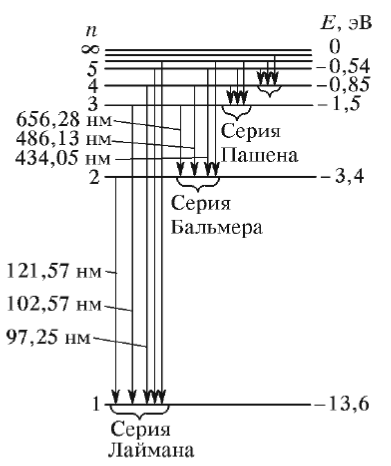
\includegraphics[width=0.3\linewidth]{img1.png}
\caption{Уровни энергии атома водорода и образование спектральныъ серий}
\label{img1}
\end{figure}

В данной работе изучается серия Бальмера, линии которой лежат в видимой области, и изотропический сдвиг меджу линиями водорода и дейтерия. Для серии Бальмера $n=2$. Величина $m$ для первых 4 линий этой серии принимает значение 3, 4, 5, 6. Эти линии обозначаются $H_\alpha, H_\beta, H_\gamma, H_\delta$.

Оценим энергии основного и возбужденного состояний атома водорода. Чтобы найти основное состояние квантовой системы, надо минимизировать, с учетом соотношения
неопределенностей, полную энергию. Потенциальная энергия электрона равна кулоновской энергии электрона в поле ядра с зарядом. Так как электрон локализован в области размером , то его импульс $p\approx\hbar/r$, и полная энергия определяется выражением:
\begin{equation}
    E=\frac{-Ze^2}{r}+\frac{\hbar^2}{2m_er^2}
\end{equation}

Условие для минимального значения энергии:
\begin{equation}
    r_\text{Б} = \frac{\hbar^2}{Zm_ee^2}
\end{equation}


Это значение боровского радиуса (радиуса первой орбиты) для электрона в поле ядра с зарядом $Z$. Энергия основного состояния:
\begin{equation}
    E=-\frac{m_ee^4}{2\hbar^2}Z^2=-RZ^2
\end{equation}

Если радиус орбиты равен $r$, то $n$-му состоянию электрона соответствует условие:
$$
2\pi r=\lambda n \quad (n=1,2,3...), \text{или} \quad m_ev_n=\frac{nh}{2\pi r}
$$
Полученное соотношение полностью совпадает со вторым постулатом Бора.

\subsection{Экспериментальная установка}

Для измерения длин волн спектральных линий в работе используется стеклянно-призменный монохроматор-спектрометр УМ-2, предназначенный для спектральных исследований в диапазоне от 0,38 до 1,00 мкм.

Призменный монохроматор УМ-2. В состав прибора УМ-2 входят следующие основные части (рис. 2):

1. Входная щель 1, снабженная микрометрическим винтом 9, который позволяет открывать щель на нужную ширину. Обычная ширина щели равна 0,02--0,03 мм.

2. Коллиматорный объектив 2, снабженный микрометрическим винтом 8. Винт позволяет смещать объектив относительно щели при фокусировке спектральных линий различных цветов.

3. Сложная спектральная призма 3, установленная на поворотном столике 6. Призма 3 состоит из трех склеенных призм $\Pi_1$, $\Pi_2$, и $\Pi_3$. Первые две призмы с преломляющими углами 30° изготовлены из тяжелого флинта, обладающего большой дисперсией. Промежуточная призма $\Pi_3$ сделана из крона. Лучи отражаются от ее гипотенузной грани и поворачиваются на 90°. Благодаря такому устройству дисперсии призм $\Pi_1$ и $\Pi_2$ складываются.

4. Поворотный столик 6, вращающийся вокруг вертикальной оси при помощи микрометрического винта 7 с отсчетным барабаном. На барабан нанесена винтовая дорожка с градусными делениями. Вдоль дорожки скользит указатель барабана. При вращении барабана призма поворачивается, и в центре поля зрения появляются различные участки спектра.

5. Зрительная труба, состоящая из объектива 4 и окуляра 5. Объектив создает изображение входной щели 1 различных цветов в своей фокальной плоскости. В этой же плоскости расположен указатель 10. Изображение щели рассматривается через окуляр 5. В случае необходимости окуляр может быть заменен выходной щелью, пропускающей одну из линий спектра. В этом случае прибор служит монохроматором.

6. Массивный корпус 11, предохраняющий прибор от повреждений и загрязнений.

\begin{figure}[h]
\centering
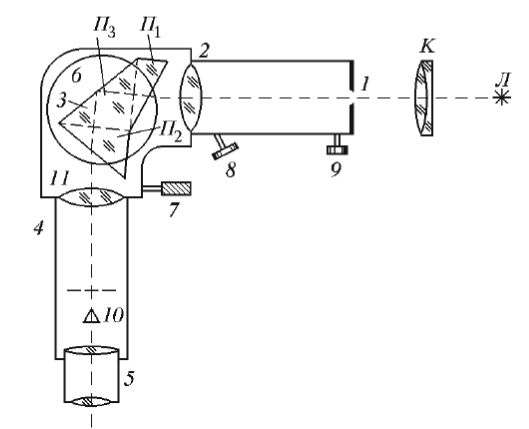
\includegraphics[width=0.5\linewidth]{img2.png}
\caption{Устройство монохроматора УМ-2}
\label{img2}
\end{figure}

7. Оптическая скамья, на которой могут перемещаться рейтеры с источником света Л и конденсором К, служащим для концентрации света на входной щели. Источник света рекомендуется располагать на расстоянии 40--50 см от щели, а конденсор -- на расстоянии 10--13 см от источника.

8. Пульт управления, служащий для питания источников света и осветительной системы спектрометра. На пульте имеются гнезда для подключения осветителей (3,5 В), неоновой лампы и лампы накаливания. Тумблеры позволяют включать лампочки осветителей шкал и указателя спектральных линий. Яркость освещения указателя регулируется реостатом.

При подготовке УМ-2 к наблюдениям особое внимание следует обращать на тщательную фокусировку, чтобы указатель 10 и спектральные линии имели четкие, ясные границы. Фокусировка производится в следующем порядке. Перемещая окуляр, следует получить резкое изображение острия указателя 10. Осветив входную щель прибора ртутной лампой, нужно найти одну из спектральных линий и получить ее резкое изображение при помощи микрометрического винта 8. При проведении измерений в другой части спектра эта операция по фокусировке должна проводиться вновь.

Для отсчета положения спектральной линии ее центр совмещается с острием указателя. Отсчет проводится по делениям барабана. Для уменьшения ошибки ширину входной щели делают по возможности малой (0,01--0,02 мм по микрометрической шкале). Для наблюдения самых слабых линий в крайней фиолетовой области щель приходится несколько расширять (до 0,03--0,05 мм). Глаз лучше замечает слабые линии в движении, поэтому при наблюдении полезно слегка поворачивать барабан в обе стороны от среднего положения.

Спектрометр УМ-2 нуждается в предварительной градуировке. Для градуировки в коротковолновой части спектра удобно применять ртутную лампу ПРК-4, а в длинноволновой и средней части спектра -- неоновую лампу. Таблицы спектральных линий ртути и неона с визуальной оценкой их относительной интенсивности приведены в Приложении V.

Градуировочную кривую следует строить в крупном масштабе на листе миллиметровой бумаги. По оси $x$ откладываются градусные деления барабана, а по оси $y$ -- длины волн соответствующих линий. Иногда при построении графика некоторые экспериментальные точки оказываются смещенными от плавной кривой. Чаще всего такие «выбросы» свидетельствуют о неправильной расшифровке наблюдаемой картины спектральных линий (главным образом, для неона). В этом случае необходимо более внимательно сопоставить картину с таблицей и внести в градуировочный график необходимые исправления.

Водородная лампа. В опытах по измерению длин волн бальмеровской серии источником света служит водородная трубка Н-образной формы, питаемая от катушки Румкорфа. Наибольшая яркость спектра достигается в том случае, когда источником света служит торец горизонтальной части трубки (капилляра).

Для увеличения яркости интересующих нас линий атомарного водорода в состав газа, которым заполняют трубку при ее изготовлении, добавляют пары воды. Молекулы воды в электрическом разряде разлагаются, образуя атомарный водород. Трубка заполняется газом до давления 5--10 Тор.

\subsection{Ход работы}
\begin{enumerate}
    \item Построим градуировочный график:

    \begin{figure}[h]
    \centering
    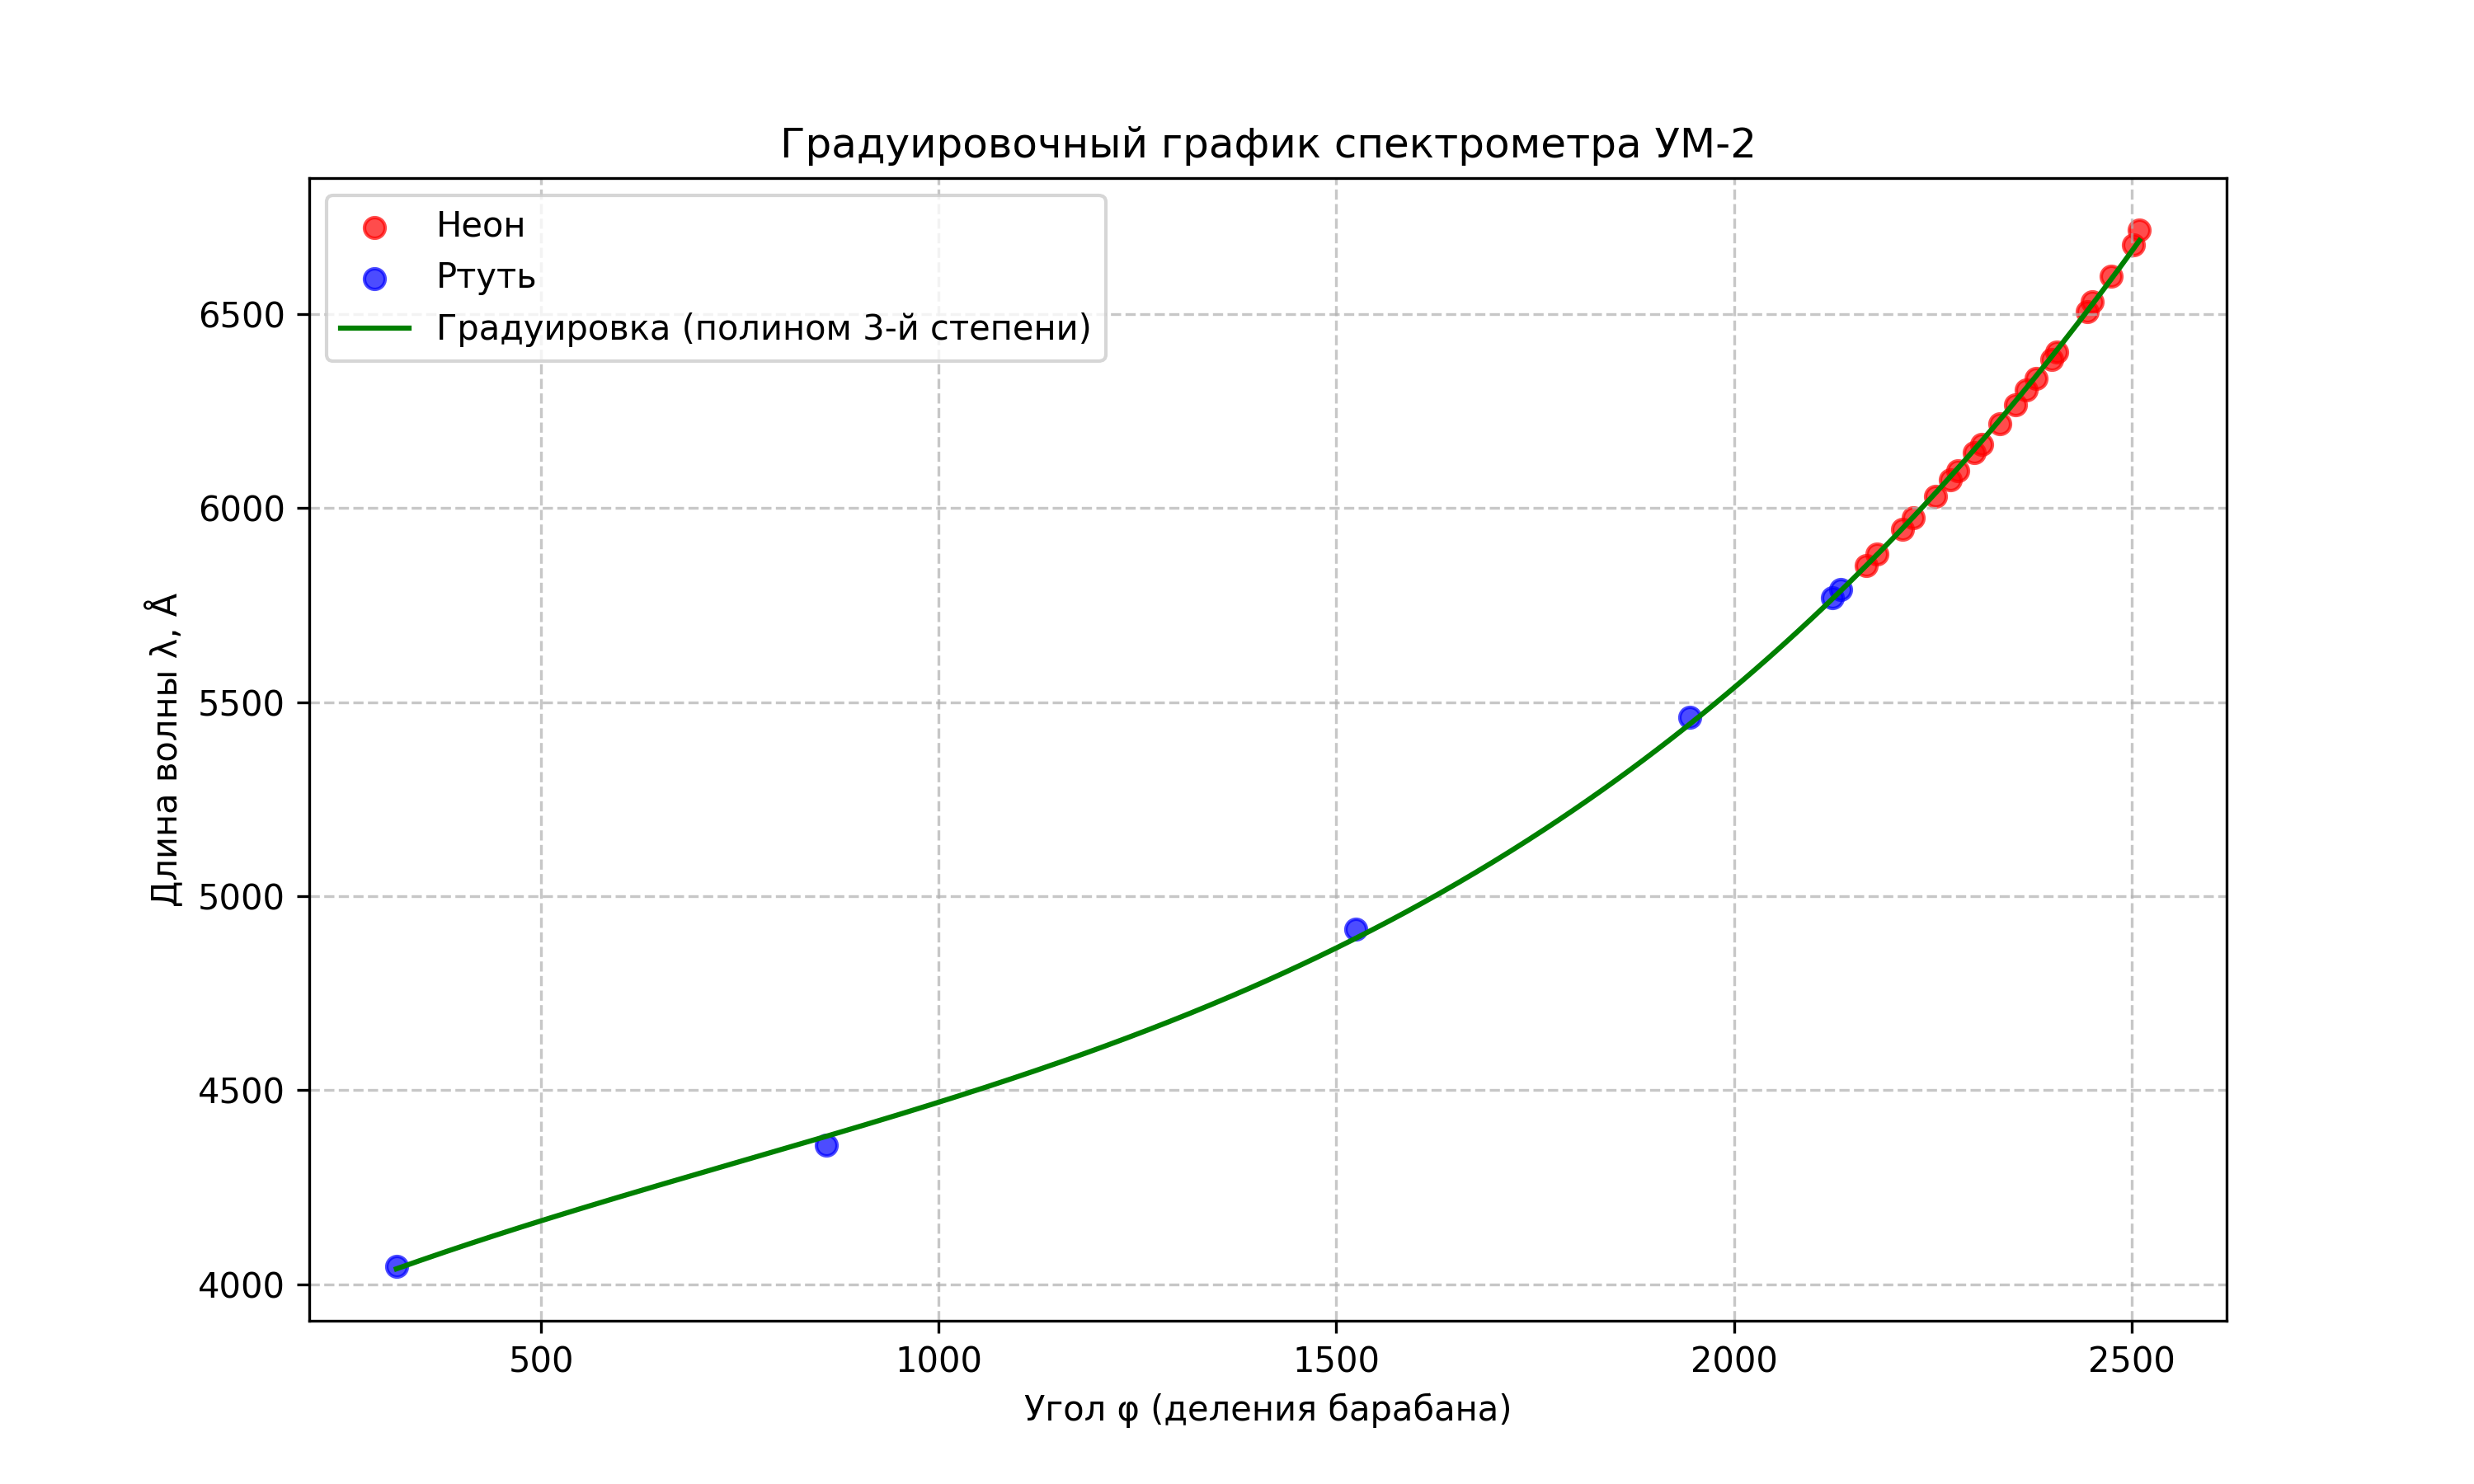
\includegraphics[width=\linewidth]{graph1.png}
    \label{img2}
    \end{figure}

    \item Измерим положение линий $H_\alpha, H_\beta, H_\gamma, H_\delta$ и с помощью калибровочного графика определим их длины волн:

    \begin{table}[h!]
    \centering
    \begin{tabular}{||c|c|c|c||}
    \hline
    $H_\alpha$ & $H_\beta$ & $H_\gamma$ & $H_\delta$ \\
    \hline
    2466 & не видим & 1472 & 836 \\
    \hline
    \hline
    $\lambda_\alpha$ & $\lambda_\beta$ & $\lambda_\gamma$ & $\lambda_\delta$ \\
    \hline
    656.7 & -- & 483.88 & 436.75 \\
    \hline
    \end{tabular}
    \end{table}

    \item Убедимся, что отношение длин волн водородных линий соответствует формуле:
    $$
    \frac{1}{\lambda_{mn}}=RZ^2\Big(\frac{1}{n^2}-\frac{1}{m^2}\Big)
    $$
    Для серии Бальмера, наблюдаемой в данной работе, $n = 2$. Линии $H_\alpha$, $H_\beta$, $H_\gamma$, $H_\delta$ соответствуют переходам с $m = 3, 4, 5, 6$ соответственно.

    Отношение длин волн двух линий должно быть обратно пропорционально отношению разностей $\left( \frac{1}{n^2} - \frac{1}{m^2} \right)$.
    
    Вычислим теоретические отношения длин волн линий $H_\gamma$ и $H_\delta$ к длине волны $H_\alpha$, приняв её за эталон.
    
    \begin{itemize}
        \item Для $H_\alpha$ ($m=3$): $\Delta_{\alpha} = \frac{1}{2^2} - \frac{1}{3^2} = \frac{1}{4} - \frac{1}{9} = \frac{5}{36}$
        \item Для $H_\gamma$ ($m=5$): $\Delta_{\gamma} = \frac{1}{2^2} - \frac{1}{5^2} = \frac{1}{4} - \frac{1}{25} = \frac{21}{100}$
        \item Для $H_\delta$ ($m=6$): $\Delta_{\delta} = \frac{1}{2^2} - \frac{1}{6^2} = \frac{1}{4} - \frac{1}{36} = \frac{8}{36} = \frac{2}{9}$
    \end{itemize}
    
    Теоретические отношения:
    $$
    \frac{\lambda_\gamma}{\lambda_\alpha} \bigg|_{\text{теор}} = \frac{\Delta_{\alpha}}{\Delta_{\gamma}} = \frac{5/36}{21/100} = \frac{5}{36} \cdot \frac{100}{21} = \frac{500}{756} \approx 0.6614
    $$
    $$
    \frac{\lambda_\delta}{\lambda_\alpha} \bigg|_{\text{теор}} = \frac{\Delta_{\alpha}}{\Delta_{\delta}} = \frac{5/36}{2/9} = \frac{5}{36} \cdot \frac{9}{2} = \frac{45}{72} = 0.6250
    $$
    
    Экспериментальные отношения, рассчитанные по измеренным длинам волн ($\lambda_\alpha = 656.7\ \text{нм}$, $\lambda_\gamma = 483.88\ \text{нм}$, $\lambda_\delta = 436.75\ \text{нм}$):
    $$
    \frac{\lambda_\gamma}{\lambda_\alpha} \bigg|_{\text{эксп}} = \frac{483.88}{656.7} \approx 0.737
    $$
    $$
    \frac{\lambda_\delta}{\lambda_\alpha} \bigg|_{\text{эксп}} = \frac{436.75}{656.7} \approx 0.665
    $$
    
    Сведём результаты в таблицу:
    
    \begin{table}[h!]
    \centering
    \begin{tabular}{||c|c|c|c||}
    \hline
    Отношение & Теоретическое & Экспериментальное & Расхождение \\ 
    \hline
    \hline
    $\lambda_\gamma / \lambda_\alpha$ & 0.6614 & 0.737 & $\sim 11.4\%$ \\ \hline
    $\lambda_\delta / \lambda_\alpha$ & 0.6250 & 0.665 & $\sim 6.4\%$ \\ \hline
    \end{tabular}
    \end{table}

    Экспериментальные отношения длин волн водородных линий по порядку величины cоответствуют формуле Ридберга, однако наблюдаются заметные расхождения (6-11$\%$). Эти расхождения могут быть связаны с погрешностями градуировки спектрометра, особенно в фиолетовой/синей области спектра, где дисперсия велика.

    \item Для каждой из наблюдаемых линий водорода вычислим значение постоянной Ридберга $R_\text{Н}$, определим ее среднее значение по всем измерениям и оценим погрешность.

    $$
    R_H = \frac{1}{\lambda_{mn} \cdot Z^2 \cdot \left( \dfrac{1}{n^2} - \dfrac{1}{m^2} \right)}
    $$
    где для атома водорода $Z = 1$, для серии Бальмера $n = 2$.
    
    \begin{itemize}
        \item Для линии $H_\alpha$ ($m = 3$):
        $\lambda_\alpha = 656.7\ \text{нм} = 656.7 \cdot 10^{-9}\ \text{м}$
        
        $R_{H\alpha} = \dfrac{1}{656.7 \cdot 10^{-9} \cdot \Big(\dfrac{1}{2^2} - \dfrac{1}{3^2}\Big)} = \dfrac{36}{656.7 \cdot 10^{-9} \cdot 5} \approx 1.096 \cdot 10^7\ \text{м}^{-1}$
    
        \item Для линии $H_\gamma$ ($m = 5$):
        $\lambda_\gamma = 483.88\ \text{нм} = 483.88 \cdot 10^{-9}\ \text{м}$
        
        $R_{H\gamma} = \dfrac{1}{483.88 \cdot 10^{-9} \cdot \Big(\dfrac{1}{2^2} - \dfrac{1}{5^2}\Big)} = \dfrac{100}{483.88 \cdot 10^{-9} \cdot 21} \approx 0.984 \cdot 10^7\ \text{м}^{-1}$

        \item Для линии $H_\delta$ ($m = 6$):
        $\lambda_\delta = 436.75\ \text{нм} = 436.75 \cdot 10^{-9}\ \text{м}$

        $R_{H\delta} = \dfrac{1}{436.75 \cdot 10^{-9} \cdot \dfrac{1}{2^2} - \dfrac{1}{6^2}} = \dfrac{9}{436.75 \cdot 10^{-9} \cdot 2} \approx 1.030 \cdot 10^7\ \text{м}^{-1}$    
    \end{itemize}
    
    Среднее значение постоянной Ридберга:
    $$
    \bar{R_H} = \frac{R_{H\alpha} + R_{H\gamma} + R_{H\delta}}{3} = \frac{1.096 + 0.984 + 1.030}{3} \cdot 10^7 \approx 1.037 \cdot 10^7\ \text{м}^{-1}
    $$
    
    Оценка погрешности проводится как стандартное отклонение среднего:

    Вычислим квадраты отклонений от среднего:
    \begin{itemize}
        \item $(R_{H\alpha} - \bar{R_H})^2 = (1.096 - 1.037)^2 \cdot 10^{14} \approx (0.059)^2 \cdot 10^{14} \approx 0.00348 \cdot 10^{14}$
        \item $(R_{H\gamma} - \bar{R_H})^2 = (0.984 - 1.037)^2 \cdot 10^{14} \approx (-0.053)^2 \cdot 10^{14} \approx 0.00281 \cdot 10^{14}$
        \item $(R_{H\delta} - \bar{R_H})^2 = (1.030 - 1.037)^2 \cdot 10^{14} \approx (-0.007)^2 \cdot 10^{14} \approx 0.00005 \cdot 10^{14}$
    \end{itemize}
    
    Сумма квадратов отклонений:
    $$
    \sum (R_i - \bar{R_H})^2 \approx (0.00348 + 0.00281 + 0.00005) \cdot 10^{14} = 0.00634 \cdot 10^{14}
    $$
    
    Стандартное отклонение для выборки ($n = 3$):
    $$
    s = \sqrt{\frac{\sum (R_i - \bar{R_H})^2}{n-1}} = \sqrt{\frac{0.00634 \cdot 10^{14}}{2}} \approx 0.0563 \cdot 10^7\ \text{м}^{-1}
    $$
    
    Стандартная ошибка среднего:
    $$
    \Delta R_H = \frac{s}{\sqrt{n}} = \frac{0.0563 \cdot 10^7}{\sqrt{3}} \approx 0.0325 \cdot 10^7\ \text{м}^{-1}
    $$
    
    Округляем погрешность до одной значащей цифры: $\Delta R_H \approx 0.03 \cdot 10^7\ \text{м}^{-1}$. Среднее значение округляем соответственно: $\bar{R_H} \approx 1.04 \cdot 10^7\ \text{м}^{-1}$.
    
    Окончательный результат:
    $$
    R_H = (1.04 \pm 0.03) \cdot 10^7\ \text{м}^{-1}
    $$
    
    Табличное значение постоянной Ридберга для бесконечно тяжелого ядра:
    $$
    R_\infty = 1.097373 \cdot 10^7\ \text{м}^{-1}
    $$
    
    Расхождение между экспериментальным и табличным значениями:
    $$
    \delta = \frac{|R_\infty - \bar{R_H}|}{R_\infty} \cdot 100\% = \frac{|1.097 - 1.04|}{1.097} \cdot 100\% \approx 5.2\%
    $$
    
\end{enumerate}

\section{Спектр молекул йода}
В первом приближении энергия молекулы может быть представлена в виде:
$$
E = E_e + E_0 + E_r
$$
где $E_e$ - энергия электронных уровней, $E_0$ - энергия колебательньных уровней, $E_r$ - энергия вращательных уровней. Спектр молекулярного йода представлен на рисунке. Видимый спектр состоит из 0-й и 1-й серий Деландра. 2-я серия в 10 раз менее интенсивная, чем 0-я, и поэтому ей пренебрегаем.

В данной работе рассматриваются оптические переходы, то есть переходы, связанные с излучением фотонов в видимом диапазоне длин волн. Они соответсвтуют переходам между различными электронными состояниями. При этом также происходят изменения вращательного и колебательного состояний, однако в реальности ввиду малости характерных энергий вращательные переходы ненаблюдаемы.

В работе изучаются переходы из колебательного состояния с номером $n_1$ освновного электронного уровня с энергией $E_1$ в колебательное состояние с номером $n_2$ на электронный уровень с энергией $E_2$ Энергия таких переходов описывается формулой:
\begin{equation}
    h\nu_{n_1,n_2} = (E_2-E_1) + h\nu_2(n_2+\frac{1}{2})-h\nu_1(n_1+\frac{1}{2})
\end{equation}
где $\nu_1$ и $\nu_2$ суть энергии колебательных квантов на электронных уровнях с энергиями $E_1$ и $E_2$.

При достаточно больших квантовых числах $n_1$ и $n_2$ колебательные уровни переходят в непрерывный спектр, что соответствует диссоциации молекулы. Наименьшая энергия, которую нужно сообщить молекуле в нижайшем колебательном состоянии, чтобы она диссоциировала, называется \textbf{энергией диссоциации}.

\subsection{Экспериментальная установка}

\begin{figure}[h]
\centering
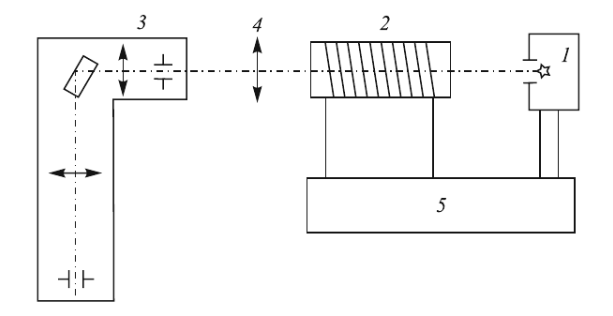
\includegraphics[width=0.6\linewidth]{img5.png}
\caption{Схема экспериментальной установки}
\label{img5}
\end{figure}

В данной работе спектр поглощения паров йода наблюдается визуально на фоне сплошного спектра лампы накаливания 1, питаемой от блока питания 5. Кювета 2 с кристаллами йода подогревается резистором, подключенным вместе с лампой накаливания к блоку питания. Линза 4 используется для формирования пучка света, проходящего через кювету, и фокусировки его на входной щели монохроматора. В результате подогрева кристаллы йода частично возгоняются, образуя пары с легкой фиолетовой окраской. Монохроматор 3 используется в качестве спектроскопа, позволяющего визуально наблюдать линии поглощения молекул йода на фоне сплошного спектра излучения лампы накаливания в видимой области.

\subsection{Ход работы}

\begin{enumerate}
    \item Определим деления барабана монохроматора, соответствующие:
    \begin{itemize}
        \item Линия $h\nu_{1,0}$ (самая длинноволновая): $n_{1,0} = 2290$
        \item Линия $h\nu_{1,5}$ (шестая от края): $n_{1,5} = 2186$
        \item Граница схождения спектра $h\nu_{\text{гр}}$: $n_{\text{гр}} = 1688$
    \end{itemize}

    \item По градуировочному графику монохроматора определим соответствующие длины волн:
    
    \begin{table}[h!]
    \centering
    \begin{tabular}{||c|c|c||}
    \hline
     & Деления барабана, $n$ & Длина волны, нм \\
    \hline
    \hline
    $h\nu_{1,0}$ & 2290 & 647.6 \\
    \hline
    $h\nu_{1,5}$ & 2186 & 632.4 \\
    \hline
    $h\nu_{\text{гр}}$ & 1688 & 557.2 \\
    \hline
    \end{tabular}
    \end{table}

    \item Вычислим энергию колебательного кванта возбужденного состояния молекулы йода:
    $$
    h\nu_2 = \frac{h\nu_{1,5} - h\nu_{1,0}}{5} = \frac{1.961 - 1.914}{5} \approx 0.0094\ \text{эВ}
    $$

    \item Используя полученные результаты, а также данные, что энергия колебательного кванта основного состояния $h\nu_1=0.027$эВ и энергия возбуждения атома $E=0.94$эВ, вычислим:
    \begin{enumerate}
        \item энергию электронного перехода $h\nu_\text{эл}$:
        $$
        h\nu_{\text{эл}} = h\nu_{1,0} + \frac{1}{2}h\nu_1 - \frac{1}{2}h\nu_2 = 1.914 + 0.0135 - 0.0047 \approx 1.923\ \text{эВ}
        $$

        \item энергию диссоциации молекулы в основном состоянии $D_1$:
        $$
        D_1 = h\nu_{\text{гр}} + E_a - \frac{1}{2}h\nu_1 = 2.225 + 0.94 - 0.0135 \approx 3.151\ \text{эВ}
        $$

        \item энергию диссоциации молекулы в возбужденном состоянии $D_2$:
        $$
        D_2 = h\nu_{\text{гр}} - h\nu_{\text{эл}} - \frac{1}{2}h\nu_2 = 2.225 - 1.923 - 0.0047 \approx 0.297\ \text{эВ}
        $$
    \end{enumerate}

    \begin{table}[h!]
    \centering
    \begin{tabular}{||c|c|c|c||}
    \hline
    Параметр & Эксперимент & Таблица & Расхождение \\
    \hline
    \hline
    $D_1$, эВ & 3.151 & 1.5425 & 104\% \\
    \hline
    $D_2$, эВ & 0.297 & 0.69 & 57\% \\
    \hline
    \end{tabular}
    \end{table}   
\end{enumerate}

\section{Выводы}

\subsection{По спектрам атома водорода}

\begin{enumerate}
    \item Экспериментально исследована серия Бальмера спектра атома водорода. Измерены длины волн линий $H_\alpha$ (656.7 нм), $H_\gamma$ (483.88 нм) и $H_\delta$ (436.75 нм). Линия $H_\beta$ не наблюдалась.

    \item Проверка соотношения длин волн показала качественное соответствие формуле Ридберга. Наблюдаемые расхождения (6-11$\%$) связаны с погрешностями измерений, особенно в сине-фиолетовой области спектра, где дисперсия монохроматора УМ-2 наибольшая.

    \item По результатам измерений вычислена постоянная Ридберга для водорода:
    $$
    R_H = (1.04 \pm 0.03) \cdot 10^7\ \text{м}^{-1}
    $$
    Расхождение с табличным значением $R_\infty = 1.097 \cdot 10^7$ м$^{-1}$ составляет 5.2\%.

    \item Наибольший вклад в погрешность внесла линия $H_\gamma$.
\end{enumerate}

\subsection{По спектру поглощения молекул йода}

\begin{enumerate}
    \item Исследован колебательно-вращательный спектр поглощения паров йода. Измерены положения характерных линий и границы схождения спектра.

    \item Определена энергия колебательного кванта возбужденного состояния: 
    \[
    h\nu_2 = 0.0094\ \text{эВ}
    \]

    \item Рассчитаны основные параметры молекулы йода:
    \begin{itemize}
        \item Энергия электронного перехода: $h\nu_{\text{эл}} = 1.923$ эВ
        \item Энергия диссоциации в основном состоянии: $D_1 = 3.151$ эВ
        \item Энергия диссоциации в возбужденном состоянии: $D_2 = 0.297$ эВ
    \end{itemize}

    \item Обнаружены значительные расхождения с табличными значениями ($D_1$ - 104\%, $D_2$ - 57\%), что может быть связано с погрешностью градуировки монохроматора в области 500-650 нм или влиянием температуры на населенность колебательных уровней.
\end{enumerate}

\subsection{Общий вывод}

В данной лабораторной работе мы увидели принципиальное различие между атомными и молекулярными спектрами. В атомных спектрах наблюдаются дискретные линии, соответствующие электронным переходам, в то время как молекулярные спектры имеют полосатую структуру, обусловленную наложением колебательных и вращательных переходов на электронные. Экспериментальные результаты неплохо согласуются с теоретическими значениями в пределах погрешностей измерений.

\end{document}
